% Created by tikzDevice version 0.10.1.2 on 2018-03-12 18:27:04
% !TEX encoding = UTF-8 Unicode
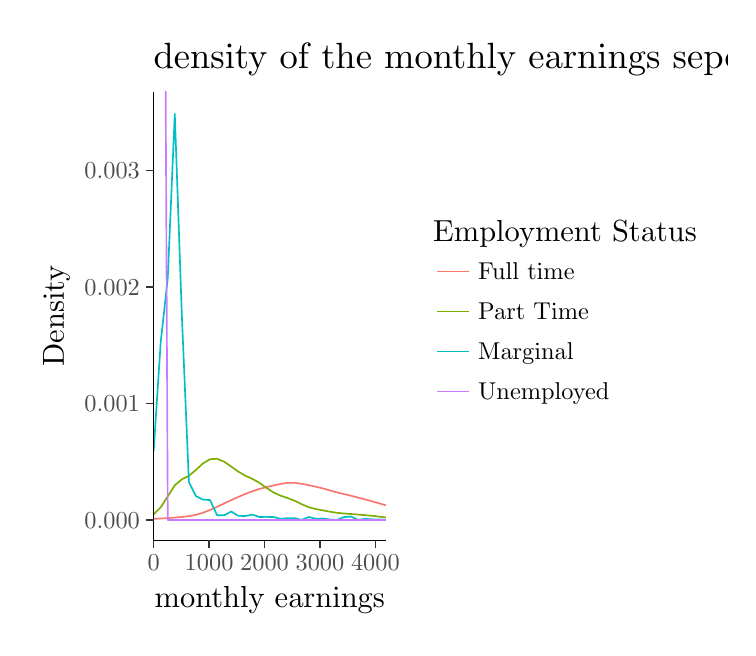
\begin{tikzpicture}[x=1pt,y=1pt]
\definecolor{fillColor}{RGB}{255,255,255}
\path[use as bounding box,fill=fillColor,fill opacity=0.00] (0,0) rectangle (252.94,216.81);
\begin{scope}
\path[clip] (  0.00,  0.00) rectangle (252.94,216.81);
\definecolor{drawColor}{RGB}{255,255,255}
\definecolor{fillColor}{RGB}{255,255,255}

\path[draw=drawColor,line width= 0.6pt,line join=round,line cap=round,fill=fillColor] (  0.00,  0.00) rectangle (252.94,216.81);
\end{scope}
\begin{scope}
\path[clip] ( 45.51, 31.53) rectangle (129.46,193.67);
\definecolor{fillColor}{RGB}{255,255,255}

\path[fill=fillColor] ( 45.51, 31.53) rectangle (129.46,193.67);
\definecolor{drawColor}{RGB}{248,118,109}

\path[draw=drawColor,line width= 0.6pt,line join=round] ( 45.52, 39.32) --
	( 48.07, 39.45) --
	( 50.62, 39.60) --
	( 53.16, 39.78) --
	( 55.71, 40.00) --
	( 58.26, 40.30) --
	( 60.81, 40.78) --
	( 63.36, 41.52) --
	( 65.90, 42.52) --
	( 68.45, 43.68) --
	( 71.00, 44.90) --
	( 73.55, 46.10) --
	( 76.10, 47.24) --
	( 78.64, 48.31) --
	( 81.19, 49.28) --
	( 83.74, 50.12) --
	( 86.29, 50.81) --
	( 88.84, 51.39) --
	( 91.39, 51.94) --
	( 93.93, 52.33) --
	( 96.48, 52.34) --
	( 99.03, 51.98) --
	(101.58, 51.47) --
	(104.13, 50.94) --
	(106.67, 50.32) --
	(109.22, 49.59) --
	(111.77, 48.89) --
	(114.32, 48.28) --
	(116.87, 47.67) --
	(119.41, 47.01) --
	(121.96, 46.33) --
	(124.51, 45.64) --
	(127.06, 44.91) --
	(129.61, 44.18) --
	(132.16, 43.60) --
	(134.70, 43.21) --
	(137.25, 42.99) --
	(139.80, 42.89) --
	(142.35, 42.88) --
	(144.90, 42.81) --
	(147.44, 42.54) --
	(149.99, 42.12) --
	(152.54, 41.71) --
	(155.09, 41.41) --
	(157.64, 41.21) --
	(160.18, 41.07) --
	(162.73, 40.97) --
	(165.28, 40.87) --
	(167.83, 40.70) --
	(170.38, 40.49) --
	(172.92, 40.29) --
	(175.47, 40.15) --
	(178.02, 40.08) --
	(180.57, 40.07) --
	(183.12, 40.09) --
	(185.67, 40.08) --
	(188.21, 40.00) --
	(190.76, 39.89) --
	(193.31, 39.83) --
	(195.86, 39.80) --
	(198.41, 39.80) --
	(200.95, 39.82) --
	(203.50, 39.88) --
	(206.05, 39.87) --
	(208.60, 39.72) --
	(211.15, 39.50) --
	(213.69, 39.33) --
	(216.24, 39.23) --
	(218.79, 39.17) --
	(221.34, 39.13) --
	(223.89, 39.11) --
	(226.44, 39.09) --
	(228.98, 39.08) --
	(231.53, 39.09) --
	(234.08, 39.12) --
	(236.63, 39.17) --
	(239.18, 39.23) --
	(241.72, 39.31) --
	(244.27, 39.36) --
	(246.82, 39.33) --
	(249.37, 39.23) --
	(251.92, 39.10) --
	(252.94, 39.06);
\definecolor{drawColor}{RGB}{124,174,0}

\path[draw=drawColor,line width= 0.6pt,line join=round] ( 45.52, 40.97) --
	( 48.07, 43.48) --
	( 50.62, 47.46) --
	( 53.16, 51.45) --
	( 55.71, 53.60) --
	( 58.26, 54.90) --
	( 60.81, 56.99) --
	( 63.36, 59.37) --
	( 65.90, 60.87) --
	( 68.45, 61.02) --
	( 71.00, 59.97) --
	( 73.55, 58.22) --
	( 76.10, 56.38) --
	( 78.64, 54.92) --
	( 81.19, 53.77) --
	( 83.74, 52.33) --
	( 86.29, 50.52) --
	( 88.84, 48.86) --
	( 91.39, 47.68) --
	( 93.93, 46.83) --
	( 96.48, 45.86) --
	( 99.03, 44.62) --
	(101.58, 43.53) --
	(104.13, 42.86) --
	(106.67, 42.39) --
	(109.22, 41.91) --
	(111.77, 41.50) --
	(114.32, 41.25) --
	(116.87, 41.07) --
	(119.41, 40.87) --
	(121.96, 40.65) --
	(124.51, 40.42) --
	(127.06, 40.13) --
	(129.61, 39.80) --
	(132.16, 39.60) --
	(134.70, 39.52) --
	(137.25, 39.45) --
	(139.80, 39.34) --
	(142.35, 39.23) --
	(144.90, 39.16) --
	(147.44, 39.11) --
	(149.99, 39.10) --
	(152.54, 39.13) --
	(155.09, 39.13) --
	(157.64, 39.08) --
	(160.18, 39.06) --
	(162.73, 39.10) --
	(165.28, 39.14) --
	(167.83, 39.09) --
	(170.38, 38.99) --
	(172.92, 38.93) --
	(175.47, 38.93) --
	(178.02, 38.95) --
	(180.57, 38.97) --
	(183.12, 38.99) --
	(185.67, 39.00) --
	(188.21, 38.97) --
	(190.76, 38.93) --
	(193.31, 38.91) --
	(195.86, 38.91) --
	(198.41, 38.94) --
	(200.95, 38.99) --
	(203.50, 39.04) --
	(206.05, 39.04) --
	(208.60, 39.00) --
	(211.15, 38.96) --
	(213.69, 38.95) --
	(216.24, 38.94) --
	(218.79, 38.93) --
	(221.34, 38.91) --
	(223.89, 38.90) --
	(226.44, 38.90) --
	(228.98, 38.90) --
	(231.53, 38.90) --
	(234.08, 38.90) --
	(236.63, 38.90) --
	(239.18, 38.91) --
	(241.72, 38.92) --
	(244.27, 38.94) --
	(246.82, 38.94) --
	(249.37, 38.93) --
	(251.92, 38.91) --
	(252.94, 38.91);
\definecolor{drawColor}{RGB}{0,191,196}

\path[draw=drawColor,line width= 0.6pt,line join=round] ( 45.52, 63.85) --
	( 48.07,103.12) --
	( 50.62,126.32) --
	( 53.16,185.66) --
	( 55.71,112.87) --
	( 58.26, 52.61) --
	( 60.81, 47.53) --
	( 63.36, 46.28) --
	( 65.90, 46.10) --
	( 68.45, 40.62) --
	( 71.00, 40.59) --
	( 73.55, 41.97) --
	( 76.10, 40.40) --
	( 78.64, 40.35) --
	( 81.19, 40.87) --
	( 83.74, 39.99) --
	( 86.29, 40.04) --
	( 88.84, 39.98) --
	( 91.39, 39.30) --
	( 93.93, 39.60) --
	( 96.48, 39.53) --
	( 99.03, 38.97) --
	(101.58, 39.99) --
	(104.13, 39.35) --
	(106.67, 39.45) --
	(109.22, 39.09) --
	(111.77, 38.94) --
	(114.32, 39.97) --
	(116.87, 40.14) --
	(119.41, 38.96) --
	(121.96, 39.31) --
	(124.51, 39.15) --
	(127.06, 39.11) --
	(129.61, 38.90) --
	(132.16, 39.09) --
	(134.70, 39.17) --
	(137.25, 38.91) --
	(139.80, 38.90) --
	(142.35, 38.90) --
	(144.90, 38.90) --
	(147.44, 38.90) --
	(149.99, 38.90) --
	(152.54, 38.90) --
	(155.09, 38.90) --
	(157.64, 38.90) --
	(160.18, 39.10) --
	(162.73, 39.45) --
	(165.28, 39.47) --
	(167.83, 38.99) --
	(170.38, 38.90) --
	(172.92, 38.90) --
	(175.47, 39.32) --
	(178.02, 38.95) --
	(180.57, 38.90) --
	(183.12, 38.90) --
	(185.67, 38.90) --
	(188.21, 38.90) --
	(190.76, 38.90) --
	(193.31, 38.90) --
	(195.86, 38.90) --
	(198.41, 38.90) --
	(200.95, 38.90) --
	(203.50, 38.90) --
	(206.05, 38.90) --
	(208.60, 38.90) --
	(211.15, 38.90) --
	(213.69, 38.90) --
	(216.24, 38.90) --
	(218.79, 38.90) --
	(221.34, 38.90) --
	(223.89, 38.90) --
	(226.44, 38.90) --
	(228.98, 38.90) --
	(231.53, 38.90) --
	(234.08, 38.90) --
	(236.63, 38.90) --
	(239.18, 38.90) --
	(241.72, 38.90) --
	(244.27, 38.90) --
	(246.82, 38.90) --
	(249.37, 38.90) --
	(251.92, 38.90) --
	(252.94, 38.90);
\definecolor{drawColor}{RGB}{199,124,255}

\path[draw=drawColor,line width= 0.6pt,line join=round] ( 49.75,216.81) --
	( 50.62, 38.90) --
	( 53.16, 38.90) --
	( 55.71, 38.90) --
	( 58.26, 38.90) --
	( 60.81, 38.90) --
	( 63.36, 38.90) --
	( 65.90, 38.90) --
	( 68.45, 38.90) --
	( 71.00, 38.90) --
	( 73.55, 38.90) --
	( 76.10, 38.90) --
	( 78.64, 38.90) --
	( 81.19, 38.90) --
	( 83.74, 38.90) --
	( 86.29, 38.90) --
	( 88.84, 38.90) --
	( 91.39, 38.90) --
	( 93.93, 38.90) --
	( 96.48, 38.90) --
	( 99.03, 38.90) --
	(101.58, 38.90) --
	(104.13, 38.90) --
	(106.67, 38.90) --
	(109.22, 38.90) --
	(111.77, 38.90) --
	(114.32, 38.90) --
	(116.87, 38.90) --
	(119.41, 38.90) --
	(121.96, 38.90) --
	(124.51, 38.90) --
	(127.06, 38.90) --
	(129.61, 38.90) --
	(132.16, 38.90) --
	(134.70, 38.90) --
	(137.25, 38.90) --
	(139.80, 38.90) --
	(142.35, 38.90) --
	(144.90, 38.90) --
	(147.44, 38.90) --
	(149.99, 38.90) --
	(152.54, 38.90) --
	(155.09, 38.90) --
	(157.64, 38.90) --
	(160.18, 38.90) --
	(162.73, 38.90) --
	(165.28, 38.90) --
	(167.83, 38.90) --
	(170.38, 38.90) --
	(172.92, 38.90) --
	(175.47, 38.90) --
	(178.02, 38.90) --
	(180.57, 38.90) --
	(183.12, 38.90) --
	(185.67, 38.90) --
	(188.21, 38.90) --
	(190.76, 38.90) --
	(193.31, 38.90) --
	(195.86, 38.90) --
	(198.41, 38.90) --
	(200.95, 38.90) --
	(203.50, 38.90) --
	(206.05, 38.90) --
	(208.60, 38.90) --
	(211.15, 38.90) --
	(213.69, 38.90) --
	(216.24, 38.90) --
	(218.79, 38.90) --
	(221.34, 38.90) --
	(223.89, 38.90) --
	(226.44, 38.90) --
	(228.98, 38.90) --
	(231.53, 38.90) --
	(234.08, 38.90) --
	(236.63, 38.90) --
	(239.18, 38.90) --
	(241.72, 38.90) --
	(244.27, 38.90) --
	(246.82, 38.90) --
	(249.37, 38.90) --
	(251.92, 38.90) --
	(252.94, 38.90);
\end{scope}
\begin{scope}
\path[clip] (  0.00,  0.00) rectangle (252.94,216.81);
\definecolor{drawColor}{RGB}{0,0,0}

\path[draw=drawColor,line width= 0.6pt,line join=round] ( 45.51, 31.53) --
	( 45.51,193.67);
\end{scope}
\begin{scope}
\path[clip] (  0.00,  0.00) rectangle (252.94,216.81);
\definecolor{drawColor}{gray}{0.30}

\node[text=drawColor,anchor=base east,inner sep=0pt, outer sep=0pt, scale=  0.88] at ( 40.56, 35.87) {0.000};

\node[text=drawColor,anchor=base east,inner sep=0pt, outer sep=0pt, scale=  0.88] at ( 40.56, 77.99) {0.001};

\node[text=drawColor,anchor=base east,inner sep=0pt, outer sep=0pt, scale=  0.88] at ( 40.56,120.10) {0.002};

\node[text=drawColor,anchor=base east,inner sep=0pt, outer sep=0pt, scale=  0.88] at ( 40.56,162.22) {0.003};
\end{scope}
\begin{scope}
\path[clip] (  0.00,  0.00) rectangle (252.94,216.81);
\definecolor{drawColor}{gray}{0.20}

\path[draw=drawColor,line width= 0.6pt,line join=round] ( 42.76, 38.90) --
	( 45.51, 38.90);

\path[draw=drawColor,line width= 0.6pt,line join=round] ( 42.76, 81.02) --
	( 45.51, 81.02);

\path[draw=drawColor,line width= 0.6pt,line join=round] ( 42.76,123.13) --
	( 45.51,123.13);

\path[draw=drawColor,line width= 0.6pt,line join=round] ( 42.76,165.25) --
	( 45.51,165.25);
\end{scope}
\begin{scope}
\path[clip] (  0.00,  0.00) rectangle (252.94,216.81);
\definecolor{drawColor}{RGB}{0,0,0}

\path[draw=drawColor,line width= 0.6pt,line join=round] ( 45.51, 31.53) --
	(129.46, 31.53);
\end{scope}
\begin{scope}
\path[clip] (  0.00,  0.00) rectangle (252.94,216.81);
\definecolor{drawColor}{gray}{0.20}

\path[draw=drawColor,line width= 0.6pt,line join=round] ( 45.52, 28.78) --
	( 45.52, 31.53);

\path[draw=drawColor,line width= 0.6pt,line join=round] ( 65.55, 28.78) --
	( 65.55, 31.53);

\path[draw=drawColor,line width= 0.6pt,line join=round] ( 85.58, 28.78) --
	( 85.58, 31.53);

\path[draw=drawColor,line width= 0.6pt,line join=round] (105.62, 28.78) --
	(105.62, 31.53);

\path[draw=drawColor,line width= 0.6pt,line join=round] (125.65, 28.78) --
	(125.65, 31.53);
\end{scope}
\begin{scope}
\path[clip] (  0.00,  0.00) rectangle (252.94,216.81);
\definecolor{drawColor}{gray}{0.30}

\node[text=drawColor,anchor=base,inner sep=0pt, outer sep=0pt, scale=  0.88] at ( 45.52, 20.52) {0};

\node[text=drawColor,anchor=base,inner sep=0pt, outer sep=0pt, scale=  0.88] at ( 65.55, 20.52) {1000};

\node[text=drawColor,anchor=base,inner sep=0pt, outer sep=0pt, scale=  0.88] at ( 85.58, 20.52) {2000};

\node[text=drawColor,anchor=base,inner sep=0pt, outer sep=0pt, scale=  0.88] at (105.62, 20.52) {3000};

\node[text=drawColor,anchor=base,inner sep=0pt, outer sep=0pt, scale=  0.88] at (125.65, 20.52) {4000};
\end{scope}
\begin{scope}
\path[clip] (  0.00,  0.00) rectangle (252.94,216.81);
\definecolor{drawColor}{RGB}{0,0,0}

\node[text=drawColor,anchor=base,inner sep=0pt, outer sep=0pt, scale=  1.10] at ( 87.49,  7.44) {monthly earnings};
\end{scope}
\begin{scope}
\path[clip] (  0.00,  0.00) rectangle (252.94,216.81);
\definecolor{drawColor}{RGB}{0,0,0}

\node[text=drawColor,rotate= 90.00,anchor=base,inner sep=0pt, outer sep=0pt, scale=  1.10] at ( 13.08,112.60) {Density};
\end{scope}
\begin{scope}
\path[clip] (  0.00,  0.00) rectangle (252.94,216.81);
\definecolor{fillColor}{RGB}{255,255,255}

\path[fill=fillColor] (140.84, 72.41) rectangle (247.44,152.80);
\end{scope}
\begin{scope}
\path[clip] (  0.00,  0.00) rectangle (252.94,216.81);
\definecolor{drawColor}{RGB}{0,0,0}

\node[text=drawColor,anchor=base west,inner sep=0pt, outer sep=0pt, scale=  1.10] at (146.54,139.53) {Employment Status};
\end{scope}
\begin{scope}
\path[clip] (  0.00,  0.00) rectangle (252.94,216.81);
\definecolor{drawColor}{RGB}{248,118,109}

\path[draw=drawColor,line width= 0.6pt,line join=round] (147.98,128.69) -- (159.54,128.69);
\end{scope}
\begin{scope}
\path[clip] (  0.00,  0.00) rectangle (252.94,216.81);
\definecolor{drawColor}{RGB}{124,174,0}

\path[draw=drawColor,line width= 0.6pt,line join=round] (147.98,114.24) -- (159.54,114.24);
\end{scope}
\begin{scope}
\path[clip] (  0.00,  0.00) rectangle (252.94,216.81);
\definecolor{drawColor}{RGB}{0,191,196}

\path[draw=drawColor,line width= 0.6pt,line join=round] (147.98, 99.78) -- (159.54, 99.78);
\end{scope}
\begin{scope}
\path[clip] (  0.00,  0.00) rectangle (252.94,216.81);
\definecolor{drawColor}{RGB}{199,124,255}

\path[draw=drawColor,line width= 0.6pt,line join=round] (147.98, 85.33) -- (159.54, 85.33);
\end{scope}
\begin{scope}
\path[clip] (  0.00,  0.00) rectangle (252.94,216.81);
\definecolor{drawColor}{RGB}{0,0,0}

\node[text=drawColor,anchor=base west,inner sep=0pt, outer sep=0pt, scale=  0.88] at (162.80,125.66) {Full time};
\end{scope}
\begin{scope}
\path[clip] (  0.00,  0.00) rectangle (252.94,216.81);
\definecolor{drawColor}{RGB}{0,0,0}

\node[text=drawColor,anchor=base west,inner sep=0pt, outer sep=0pt, scale=  0.88] at (162.80,111.20) {Part Time};
\end{scope}
\begin{scope}
\path[clip] (  0.00,  0.00) rectangle (252.94,216.81);
\definecolor{drawColor}{RGB}{0,0,0}

\node[text=drawColor,anchor=base west,inner sep=0pt, outer sep=0pt, scale=  0.88] at (162.80, 96.75) {Marginal};
\end{scope}
\begin{scope}
\path[clip] (  0.00,  0.00) rectangle (252.94,216.81);
\definecolor{drawColor}{RGB}{0,0,0}

\node[text=drawColor,anchor=base west,inner sep=0pt, outer sep=0pt, scale=  0.88] at (162.80, 82.30) {Unemployed};
\end{scope}
\begin{scope}
\path[clip] (  0.00,  0.00) rectangle (252.94,216.81);
\definecolor{drawColor}{RGB}{0,0,0}

\node[text=drawColor,anchor=base west,inner sep=0pt, outer sep=0pt, scale=  1.32] at ( 45.51,202.22) {density of the monthly earnings seperated by employment status };
\end{scope}
\end{tikzpicture}
